\section{Julia编译流程}
\label{sec:julia:complier_process}
 \paragraph{Julia}的编译可以分为几个阶段,通过宏我们可以看到在每个阶段Julia编译器分别做了什么。来看下面这段代码:
  \begin{lstlisting}
function vsum(x)
    sum = 0
    for i = 1:length(x)
        @inbounds v = x[i]
        if !is_na(v)
            sum += v
        end
    end
    sum
end
\end{lstlisting}
直接使用@code\_native宏查看在我的电脑中的生成的汇编结果
\begin{lstlisting}
@code_native vsum(1)
...... // 省略
\end{lstlisting}
发现已经自动进行了内联,这与C语言有很大的不同,再使用@code\_llvm宏查看上一层次的代码,即它的llvm ir代码:
\begin{lstlisting}
@code_llvm vsum(1)
...... // 省略
\end{lstlisting}
通过llvm ir的代码可以看到在生成llvm ir的时候也已经完成了内联,这个时候想起论文\cite{bezanson2018Julia}
(\href{https://dl.acm.org/citation.cfm?id=3276490}{OOPSLA2018}, 
\S\ref{paper:oopsla2018Julia})上的一张图片:

\begin{figure}[h]  
\centering
\subfigure[A given traffic flow set]{
  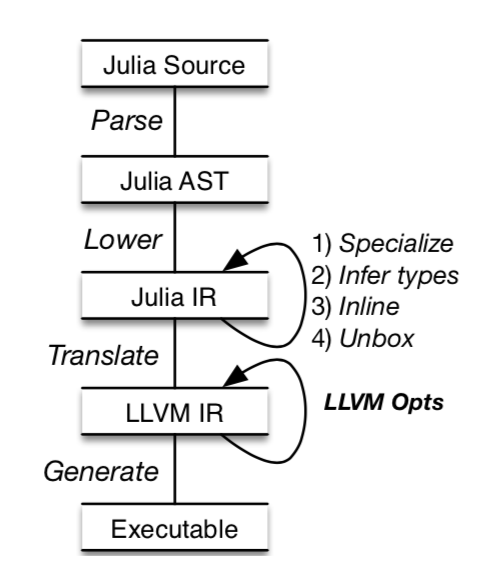
\includegraphics[width=2.2in]{oop4.png}}
\caption{编译流程图}
\end{figure}

看来在更早之前就完成了特化、类型推断、内联、拆箱的工作,经过查找发现有几个指令可以得到对应的阶段代码。
首先是@code\_lowered宏,它把源代码转化为类似于Python byte code的形式,这种形式的一个特点是single static assignment,意思是每个变量只赋值一次,并且每个变量都要先声明,再使用,此外,循环和条件语句被转化为goto和label的组合形式。

\begin{lstlisting}
julia> @code_lowered vsum(1)  // like python byte code
CodeInfo(
2 1 ─       sum = 0                                                         │
3 │   %2  = (Main.length)(x)                                                │
  │   %3  = 1:%2                                                            │
  │         #temp# = (Base.iterate)(%3)                                     │
  │   %5  = #temp# === nothing                                              │
  │   %6  = (Base.not_int)(%5)                                              │
  └──       goto #6 if not %6                                               │
  2 ┄ %8  = #temp#                                                          │
  │         i = (Core.getfield)(%8, 1)                                      │
  │   %10 = (Core.getfield)(%8, 2)                                          │
4 │         $(Expr(:inbounds, true))                                        │
  │   %12 = (Base.getindex)(x, i)                                           │
  │         v = %12                                                         │
  │         val = %12                                                       │
  │         $(Expr(:inbounds, :pop))                                        │
  │         val                                                             │
5 │   %17 = (Main.is_na)(v)                                                 │
  │   %18 = !%17                                                            │
  └──       goto #4 if not %18                                              │
6 3 ─       sum = sum + v                                                   │
  4 ─       #temp# = (Base.iterate)(%3, %10)                                │
  │   %22 = #temp# === nothing                                              │
  │   %23 = (Base.not_int)(%22)                                             │
  └──       goto #6 if not %23                                              │
  5 ─       goto #2                                                         │
9 6 ─       return sum                                                      │
)

\end{lstlisting}

另一个是@code\_typed宏,在这个阶段我们可以看到完成了内联和类型推断
\begin{lstlisting}
julia> @code_typed vsum(1)
CodeInfo(
3 1 ──       (Base.ifelse)(true, 1, 0)::Int64                  │╻╷╷  Colon
  │    %2  = (Base.slt_int)(1, 1)::Bool                        ││╻╷╷  isempty
  └───       goto #3 if not %2                                 ││   
  2 ──       goto #4                                           ││   
  3 ──       goto #4                                           ││   
  4 ┄─ %6  = φ (#2 => true, #3 => false)::Bool                 │    
  │    %7  = φ (#3 => 1)::Int64                                │    
  │    %8  = φ (#3 => 1)::Int64                                │    
  │    %9  = (Base.not_int)(%6)::Bool                          │    
  └───       goto #22 if not %9                                │    
  5 ┄─ %11 = φ (#4 => 0, #21 => %36)::Int64                    │    
  │    %12 = φ (#4 => %7, #21 => %42)::Int64                   │    
  │    %13 = φ (#4 => %8, #21 => %43)::Int64                   │    
4 └───       goto #9 if not false                              │╻    getindex
  6 ── %15 = (%12 === 1)::Bool                                 ││╻    ==
  └───       goto #8 if not %15                                ││   
  7 ──       goto #9                                           ││   
  8 ── %18 = %new(Core.BoundsError)::BoundsError               ││╻    Type
  │          (Base.throw)(%18)::Union{}                        ││   
  └───       $(Expr(:unreachable))::Union{}                    ││   
  9 ┄─       goto #10                                          ││   
  5 10 ─ %22 = (Main.is_na)(x)::Any                              │    
  │    %23 = (isa)(%22, Missing)::Bool                         │    
  └───       goto #12 if not %23                               │    
  11 ─       goto #15                                          │    
  12 ─ %26 = (isa)(%22, Bool)::Bool                            │    
  └───       goto #14 if not %26                               │    
  13 ─ %28 = π (%22, Bool)                                     │    
  │    %29 = (Base.not_int)(%28)::Bool                         │╻    !
  └───       goto #15                                          │    
  14 ─ %31 = !%22::Union{Missing, Bool, ##54#55{_1} where _1}  │    
  └───       goto #15                                          │    
  15 ┄ %33 = φ (#11 => $(QuoteNode(missing)), #13 => %29, #14 => %31)::Union{Missing, Bool, ##54#55{_1} where _1}
  └───       goto #17 if not %33                               │    
6 16 ─ %35 = (Base.add_int)(%11, x)::Int64                     │╻    +
  17 ─ %36 = φ (#16 => %35, #15 => %11)::Int64                 │    
  │    %37 = (%13 === 1)::Bool                                 ││╻    == 
  └───       goto #19 if not %37                               ││   
  18 ─       goto #20                                          ││   
  19 ─ %40 = (Base.add_int)(%13, 1)::Int64                     ││╻    +
  └───       goto #20                                          │╻    iterate
  20 ┄ %42 = φ (#19 => %40)::Int64                             │    
  │    %43 = φ (#19 => %40)::Int64                             │    
  │    %44 = φ (#18 => true, #19 => false)::Bool               │    
  │    %45 = (Base.not_int)(%44)::Bool                         │    
  └───       goto #22 if not %45                               │    
  21 ─       goto #5                                           │    
9 22 ─ %48 = φ (#20 => %36, #4 => 0)::Int64                    │    
  └───       return %48                                        │    
) => Int64
\end{lstlisting}

以上就是Julia的编译流程
